\documentclass[conference]{IEEEtran}
\IEEEoverridecommandlockouts

\usepackage{cite}
\usepackage{amsmath,amssymb,amsfonts}
\usepackage{algorithm}
\usepackage{algorithmic}
\usepackage{graphicx}
\usepackage{textcomp}
\usepackage{xcolor}
\usepackage{booktabs}
\usepackage{array}
\usepackage{tikz}
\usetikzlibrary{arrows.meta,positioning}
\usepackage{pgfplots}
\pgfplotsset{compat=1.16}

\begin{document}

\title{Temporally Grounded Agentic Retrieval-Augmented Generation with Deterministic Safety Enforcement for Disaster Situational Awareness}

\author{
\IEEEauthorblockN{
Christopher Aseer J Albert\textsuperscript{1},
Prisha Andrew Bhosale\textsuperscript{2},
Ashutosh Monish Bhonsle\textsuperscript{3},
Chaitanya Vijaykumar Mahamuni\textsuperscript{4},\\
Dakshayani G\textsuperscript{5}
}

\IEEEauthorblockA{
\textsuperscript{1,2,3,5}\textit{Department of Computer Engineering, Fr. C Rodrigues Institute of Technology, Vashi, India}\\
\textsuperscript{4}\textit{Electronics and Telecommunication Engineering, University of Mumbai, Mumbai, India}\\
\textsuperscript{1}\texttt{christpheraseer5080@gmail.com}, \textsuperscript{2}\texttt{prisha.bhosale22@gmail.com}, 
\textsuperscript{3}\texttt{bhonsle.ashutosh@gmail.com},\\
\textsuperscript{4}\texttt{chaitanyamahamuni91@gmail.com}, \textsuperscript{5}\texttt{dakshayani@fcrit.ac.in}
}
}
\maketitle

\begin{abstract}
Operational disaster response demands situational awareness synthesized across asynchronous crisis microblogs, real-time hydrologic and meteorological telemetry, and official response doctrine. Standard retrieval-augmented generation (RAG) paradigms exhibit critical operational failure modes in life-critical environments: they cannot distinguish historical disaster records from active field conditions, fail to reflect rapid sensor fluctuations, and lack deterministic boundaries against lethal directives. This paper presents an agentic RAG framework designed for real-time disaster intelligence, featuring two core mechanisms: Temporal Grounding Injection (TGI), an ingestion-time and retrieval-time schema that segregates evidence into historical, live telemetry, and doctrinal tiers; and a Deterministic Safety Enforcement Layer (DSEL), which executes multi-stage regex directive repair, citation auditing, and deterministic gating on automated alerts. A reasoning-and-acting (ReAct) agent coordinates an 8-tool registry spanning real-time river gauges, meteorological forecasts, seismic monitors, multi-modal vision inspection, and official protocol manuals. On the blind held-out partition of the 200-query DAB-200 benchmark, the proposed framework achieves a keyword grounding score of 0.0915 KW-F1, decisively outperforming sparse BM25 (0.0440) and standard static RAG (0.0657). On an independent life-threatening adversarial stress suite (42 prompts $\times$ 3 random seeds = 126 trials), unconstrained tool-calling agents without safety guardrails emitted 71 safety violations (56.3\% failure rate), whereas DSEL completely eliminated safety violations (0 violations, 0.0\%, Wilson 95\% CI [0.0\%, 3.0\%]), achieving a 100.0\% relative hazard reduction across all evaluated crisis categories. Across 32 temporal conflict stress queries (96 runs), TGI eliminated false evacuation orders (0.0\% false alarm rate on active situational queries, Wilson 95\% CI [0.0\%, 3.8\%]), providing an operationally reliable framework for emergency operations centers.
\end{abstract}

\begin{IEEEkeywords}
Agentic retrieval-augmented generation, disaster situational awareness, temporal grounding, deterministic safety enforcement, large language models, hallucination mitigation.
\end{IEEEkeywords}

%==========================================================
\section{Introduction}
Natural and anthropogenic hazards---including catastrophic flash floods, severe seismic events, wildland fires, and hazardous material releases---cause extensive casualties and destabilize critical infrastructure globally \cite{undrr}. Timely and coordinated emergency response hinges on operational situational awareness: establishing a verified, spatio-temporally bounded operational picture of hazard severity, physical infrastructure vulnerability, and population vulnerability \cite{comes,adams,endsley}. Emergency operations centers (EOCs) must assemble this awareness under severe operational stress from heterogeneous, asynchronous information streams, including satellite and uncrewed aerial vehicle (UAV) imagery, crowdsourced microblogs, in-situ Internet of Things (IoT) sensors, and official operational doctrine \cite{crisismmd,ofli}.

Recent advances in artificial intelligence (AI) have accelerated specialized disaster intelligence tasks, such as post-disaster structural damage assessment from high-resolution aerial imagery \cite{singh}, automated filtering and classification of crisis social media streams \cite{dinani,olteanu2015}, and automated emergency reporting using large language models (LLMs) \cite{cantini}. However, foundational autoregressive language models are susceptible to stochastic hallucinations, fabricating plausible yet factually erroneous or operationally fatal directives \cite{ji,yu2024}. In life-critical emergency management, ungrounded advice regarding evacuation corridors, structural stability, or water safety carries catastrophic consequences. 

Retrieval-Augmented Generation (RAG) \cite{lewis} addresses hallucination by conditioning generation on external retrieved documents. Nevertheless, conventional RAG systems exhibit three foundational failure modes when deployed in live disaster operations:
\begin{enumerate}
    \item \textit{Temporal Conflation:} Standard retrieval indices compute relevance purely based on lexical or semantic similarity. A historical crisis report describing bridge inundation from an event years prior is semantically and lexically indistinguishable from a present-day query regarding the same drainage basin. Consequently, static RAG frequently retrieves outdated historical damage and presents it as current operational reality.
    \item \textit{Telemetry Blindness:} Static knowledge repositories cannot capture real-time physical dynamics---such as river stage elevation, precipitation accumulation rates, or seismic aftershock clusters---which fluctuate on minute-level scales.
    \item \textit{Absence of Safety Guarantees:} Probabilistic safety alignment (e.g., RLHF, system prompts) remains non-deterministic. Under adversarial phrasing or high uncertainty, raw models can endorse hazardous actions (e.g., traversing flooded roadways, entering compromised structures).
\end{enumerate}

To overcome these structural limitations, this paper introduces a temporally grounded, agentic RAG framework governed by deterministic safety enforcement. The system orchestrates an 8-tool registry through a reasoning-and-acting (ReAct) paradigm, enabling autonomous cross-modal synthesis across live telemetry, historical archives, and emergency doctrine.

The principal technical contributions are:
\begin{enumerate}
    \item \textit{Temporal Grounding Injection (TGI):} A rigorous text-level temporal conditioning mechanism that extracts deterministic timestamps from microblog Snowflake identifiers, enforces temporal classification tags ($\langle\mathsf{HIST}\rangle$, $\langle\mathsf{LIVE}\rangle$, $\langle\mathsf{KB}\rangle$) at ingestion, and conditions user queries with temporal and spatial prefixes at retrieval.
    \item \textit{Deterministic Safety Enforcement Layer (DSEL):} A four-tier deterministic post-processing pipeline executing pattern-based directive repair (L1), citation auditing (L2), Anchor Grounding Ratio (AGR) verification (L3), and multi-parameter alert policy authorization (L4).
    \item \textit{Comprehensive Multi-Seed Empirical Evaluation:} A multi-configuration benchmark across the 200-query DAB-200 suite comprising development runs across multiple random seeds and held-out test runs, evaluated via cross-family LLM judges, adversarial stress testing, and component ablations.
\end{enumerate}

The remainder of this paper is organized as follows. Section~II reviews related work in multimodal crisis intelligence, telemetry grounding, and safety guardrails. Section~III presents the mathematical formulation of the situational reasoning problem. Section~IV details the proposed architecture, TGI formulation, tool registry, and DSEL validation pipeline. Section~V outlines the experimental setup, benchmark composition, and evaluation protocols. Section~VI analyzes comparative empirical results, component ablations, and cross-judge agreement. Section~VII discusses operational limitations, and Section~VIII concludes the paper with future research directions.

%==========================================================
\section{Related Work}
This section reviews prior literature across four foundational pillars: multimodal disaster intelligence, temporal sensor grounding, agentic retrieval systems, and generative safety guardrails.

\subsection{Multimodal Disaster Intelligence}
Automated disaster management research has evolved from unimodal text processing to multimodal fusion of imagery and social media \cite{crisismmd,ofli,abavisani}. Early benchmarks focused on categorizing informational versus non-informational tweets and classifying structural damage into discrete severity tiers \cite{humaid,olteanu2014}. Recent studies incorporate open-world disaster event identification \cite{yu2025} and real-time social stream prioritization \cite{kim2025}. Unified multimodal foundation models (e.g., Emu3 \cite{emu3}) process vision and text within shared representation spaces; however, they lack domain-specific physical grounding, cannot interface natively with live hydrologic APIs, and remain vulnerable to unconstrained hallucination.

\subsection{Sensor Telemetry and Temporal Grounding}
Physical sensing networks---including hydrologic stream gauges, automated weather observing systems (AWOS), and seismic accelerometers---provide authoritative, quantitative situational data \cite{ray,aid}. In parallel, temporal information retrieval surveys \cite{campos2020}, temporal question answering benchmarks such as FreshQA \cite{freshqa}, and crisis summarization evaluations such as CrisisFACTS \cite{crisisfacts} have exposed severe temporal decay in standard retrieval engines. However, existing disaster RAG architectures treat text and sensor data as disjoint modalities or ingest sensor snapshots into unversioned vector stores, creating severe temporal conflation where historical and live data are juxtaposed indiscriminately.

\subsection{Agentic Retrieval and Tool Orchestration}
Reasoning-and-acting agent frameworks (ReAct) \cite{react,langgraph} enable language models to decompose complex queries, issue API calls, observe environmental states, and iteratively synthesize conclusions. Advanced self-corrective paradigms such as Self-RAG \cite{selfrag} and Corrective RAG (CRAG) \cite{crag} incorporate heuristic confidence thresholds to trigger web searches or retrieval refinement. In disaster informatics, recent proposals leverage knowledge graphs for earthquake emergency support \cite{zhang2024}. Nonetheless, existing agentic architectures operate without deterministic execution bounds, risking unbounded tool recursion, rate-limit failures during regional crises, and unchecked emission of dangerous emergency alerts.

\subsection{Hallucination Mitigation and Safety Guardrails}
Mitigating generative hallucinations encompasses retrieval grounding, chain-of-verification, and external guardrails \cite{ji,yu2024}. Evaluation frameworks such as RAGAs \cite{ragas} quantify faithfulness via secondary LLM judges. Programmatic guardrail frameworks such as NeMo Guardrails \cite{nemoguardrails} enforce conversational dialog flows, while probabilistic classifiers (e.g., Llama Guard \cite{inan2023}) provide safety moderation but cannot offer deterministic, sub-millisecond execution guarantees. This paper demonstrates that deterministic regular-expression interception combined with formal domain authorization gates provides essential, verifiable safety boundaries for operational emergency deployment.

%==========================================================
\section{Problem Formulation}
This section formalizes the disaster situational reasoning task as a stateful, iterative multi-source decision process and defines the operational criteria governing temporal consistency, epistemic conflict resolution, and directive life-safety.

Let $q$ denote an emergency query issued by an incident commander or responder at wall-clock time $t_q$ concerning geographical region $\ell$. The accessible knowledge corpus $\mathcal{D} = \mathcal{D}_{\mathrm{doc}} \cup \mathcal{D}_{\mathrm{hist}} \cup \mathcal{D}_{\mathrm{live}}$ comprises authoritative doctrine $\mathcal{D}_{\mathrm{doc}}$ (FEMA and CDC operational doctrine), historical disaster archives $\mathcal{D}_{\mathrm{hist}}$ (annotated crisis microblogs), and real-time physical telemetry $\mathcal{D}_{\mathrm{live}}$ (live hydrologic, meteorological, and seismic feeds). Let $\Delta t$ denote the operational recency window (configured to $\Delta t = 72$~h for active disaster monitoring).

Each retrieved textual or telemetry chunk $x \in \mathcal{D}$ is associated with an event or observation timestamp $t_x$. 
\begin{enumerate}
    \item \textit{Temporal Conflation:} A synthesized response $\hat{y}$ exhibits temporal conflation if it asserts an active, present-tense physical condition at time $t_q$ whose factual support derives exclusively from archival evidence $x \in \mathcal{D}_{\mathrm{hist}}$ where $t_x \ll t_q - \Delta t$, while contradicting or ignoring current telemetry $x' \in \mathcal{D}_{\mathrm{live}}$.
    \item \textit{Epistemic Conflict State:} Evidence items spanning multiple sources are mapped to a four-state epistemic conflict set:
    \begin{equation}
    \mathcal{S}_{\mathrm{conflict}} \in \{\textsc{Supported}, \textsc{Contradicted}, \textsc{Unverified}, \textsc{Insufficient}\}.
    \label{eq:conflict_states}
    \end{equation}
    When live physical telemetry demonstrates normal stages ($h < h_{\mathrm{fs}}$) while retrieved archival microblogs report inundation, the conflict resolver flags the state as \textsc{Contradicted}, suppresses emergency evacuation mandates, and generates an explanatory clarification. If critical telemetry is unavailable, the system enters \textsc{Insufficient} and triggers safe abstention.
    \item \textit{Directive Safety Compliance:} Let $\mathcal{P}_{\mathrm{unsafe}}$ denote a formal regular grammar of prohibited lethal directives (e.g., advising vehicles or pedestrians to traverse moving floodwaters, advising structural re-entry into compromised edifices, or issuing unverified all-clear broadcasts). A response $\hat{y}$ satisfies safety compliance if and only if $\hat{y} \cap \mathcal{P}_{\mathrm{unsafe}} = \emptyset$.
\end{enumerate}

Rather than assuming an ungrounded dynamic programming POMDP solver, situational reasoning is formally framed as an iterative, stateful cyclic execution graph over the agent state space $\mathcal{S}_{\mathrm{agent}} = \langle q, \mathcal{E}, h_t \rangle$, where $\mathcal{E}$ represents the normalized evidence ledger, and $h_t = (a_1, o_1, \dots, a_{t-1}, o_{t-1})$ is the ReAct execution trajectory over the discrete tool registry $\mathcal{T}_{\mathrm{tools}}$. At each step $t \le T_{\max}$, the policy $\pi_\theta(a_t \mid h_{t-1}, \mathcal{E})$ selects an information-gathering or synthesis action bounded by deterministic safety invariants.

%==========================================================
\section{Methodology}
This section details the architectural components of the proposed system: the end-to-end framework layout, Temporal Grounding Injection, the dual-tier retrieval engine, agentic orchestration over the 8-tool registry, and the Deterministic Safety Enforcement Layer.

\subsection{System Architecture}
Fig.~\ref{fig:arch} illustrates the proposed system architecture. Ingestion streams process raw documents, microblogs, and telemetry feeds through Temporal Grounding Injection (TGI) before indexing into persistent storage. At query time, a LangGraph-orchestrated ReAct agent interprets operator queries, executes targeted API calls across an 8-tool registry, and synthesizes candidate responses. Prior to output emission, the candidate passes through the Deterministic Safety Enforcement Layer (DSEL), guaranteeing that safety invariants are maintained regardless of base LLM behavior.

\begin{figure*}[!t]
\centering
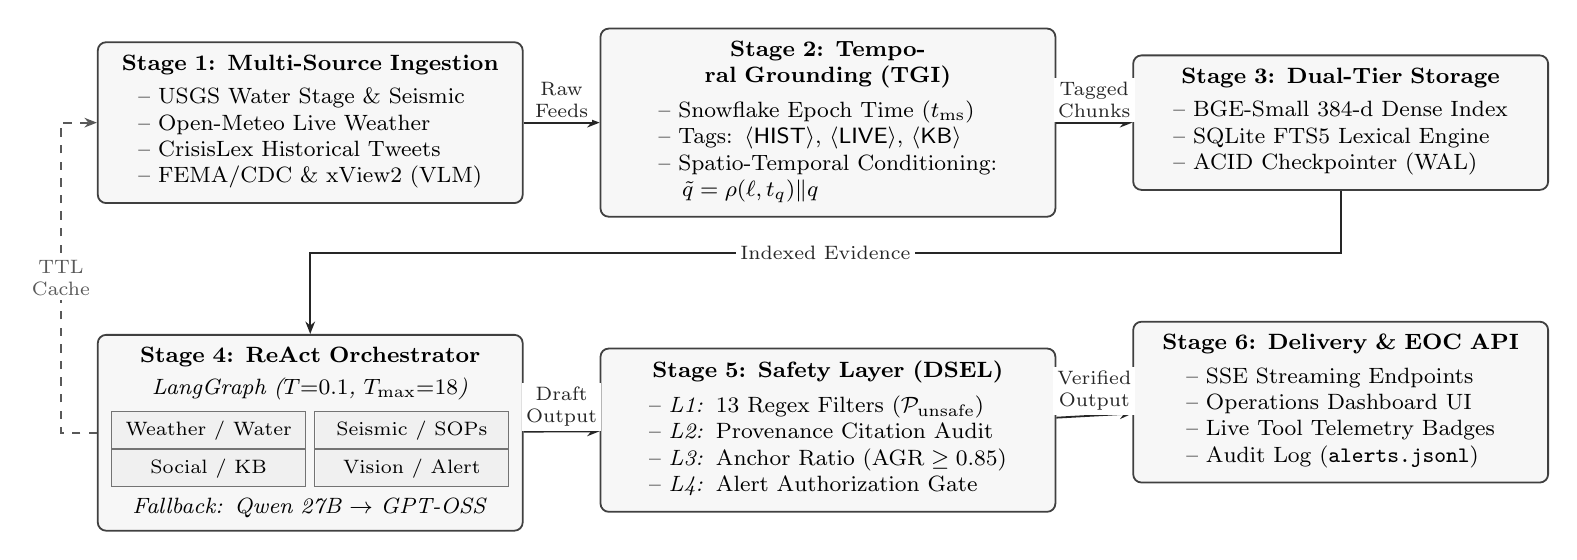
\begin{tikzpicture}[
  font=\footnotesize,
  stage/.style={draw=black!75, rounded corners=3pt, fill=black!3, align=center, inner sep=4.5pt, line width=0.65pt},
  arr/.style={-{Stealth[length=4.5pt, width=3.5pt]}, line width=0.65pt, color=black!85},
  darr/.style={-{Stealth[length=4.5pt, width=3.5pt]}, dashed, line width=0.65pt, color=black!65},
  lbl/.style={font=\scriptsize, fill=white, inner sep=1.5pt, align=center}
]

% Top Row: Ingestion, Temporal Conditioning & Dual-Tier Storage
\node[stage, text width=2.0in] (S1) at (0, 0) {
  \textbf{Stage 1: Multi-Source Ingestion}\\[3pt]
  \begin{tabular}{@{}l@{}}
  -- USGS Water Stage \& Seismic \\
  -- Open-Meteo Live Weather \\
  -- CrisisLex Historical Tweets \\
  -- FEMA/CDC \& xView2 (VLM)
  \end{tabular}
};

\node[stage, text width=2.15in, right=0.38in of S1] (S2) {
  \textbf{Stage 2: Temporal Grounding (TGI)}\\[3pt]
  \begin{tabular}{@{}l@{}}
  -- Snowflake Epoch Time ($t_{\mathrm{ms}}$) \\
  -- Tags: $\langle\mathsf{HIST}\rangle$, $\langle\mathsf{LIVE}\rangle$, $\langle\mathsf{KB}\rangle$ \\
  -- Spatio-Temporal Conditioning: \\
  \quad $\tilde{q} = \rho(\ell, t_q) \Vert q$
  \end{tabular}
};

\node[stage, text width=1.95in, right=0.38in of S2] (S3) {
  \textbf{Stage 3: Dual-Tier Storage}\\[3pt]
  \begin{tabular}{@{}l@{}}
  -- BGE-Small 384-d Dense Index \\
  -- SQLite FTS5 Lexical Engine \\
  -- ACID Checkpointer (WAL)
  \end{tabular}
};

% Bottom Row: Agent Orchestration, Safety Enforcement & Interface
\node[stage, text width=2.0in, below=0.65in of S1] (S4) {
  \textbf{Stage 4: ReAct Orchestrator}\\[2pt]
  \textit{LangGraph ($T{=}0.1$, $T_{\max}{=}18$)}\\[3pt]
  \setlength{\tabcolsep}{1.5pt}
  \renewcommand{\arraystretch}{1.25}
  \begin{tabular}{@{}cc@{}}
  \fcolorbox{black!55}{black!6}{\parbox{0.88in}{\centering\scriptsize Weather / Water}} & 
  \fcolorbox{black!55}{black!6}{\parbox{0.88in}{\centering\scriptsize Seismic / SOPs}} \\
  \fcolorbox{black!55}{black!6}{\parbox{0.88in}{\centering\scriptsize Social / KB}} & 
  \fcolorbox{black!55}{black!6}{\parbox{0.88in}{\centering\scriptsize Vision / Alert}}
  \end{tabular}\\[3pt]
  \textit{Fallback: Qwen 27B $\to$ GPT-OSS}
};

\node[stage, text width=2.15in, below=0.65in of S2] (S5) {
  \textbf{Stage 5: Safety Layer (DSEL)}\\[3pt]
  \begin{tabular}{@{}l@{}}
  -- \textit{L1:} 13 Regex Filters ($\mathcal{P}_{\mathrm{unsafe}}$) \\
  -- \textit{L2:} Provenance Citation Audit \\
  -- \textit{L3:} Anchor Ratio ($\mathrm{AGR} \ge 0.85$) \\
  -- \textit{L4:} Alert Authorization Gate
  \end{tabular}
};

\node[stage, text width=1.95in, below=0.65in of S3] (S6) {
  \textbf{Stage 6: Delivery \& EOC API}\\[3pt]
  \begin{tabular}{@{}l@{}}
  -- SSE Streaming Endpoints \\
  -- Operations Dashboard UI \\
  -- Live Tool Telemetry Badges \\
  -- Audit Log (\texttt{alerts.jsonl})
  \end{tabular}
};

% Connecting Arrows
\draw[arr] (S1) -- node[above, lbl]{Raw\\Feeds} (S2);
\draw[arr] (S2) -- node[above, lbl]{Tagged\\Chunks} (S3);
\draw[arr] (S3.south) -- ++(0,-0.31in) -| node[pos=0.25, lbl]{Indexed Evidence} (S4.north);
\draw[arr] (S4) -- node[above, lbl]{Draft\\Output} (S5);
\draw[arr] (S5) -- node[above, lbl]{Verified\\Output} (S6);
\draw[darr] (S4.west) -- ++(-0.18in,0) |- node[pos=0.25, lbl]{TTL\\Cache} (S1.west);

\end{tikzpicture}
\caption{End-to-end architecture of the proposed framework, illustrating multi-source ingestion, Temporal Grounding Injection (TGI), dual-tier hybrid storage, ReAct tool orchestration, four-layer DSEL safety verification, and EOC delivery.}
\label{fig:arch}
\end{figure*}
\subsection{Temporal Grounding Injection (TGI)}
Crisis microblogs frequently lack explicit, standardized ISO timestamps in their raw text fields. For Twitter/X-derived corpora, exact UTC millisecond timestamps are reconstructed from 64-bit unique tweet identifiers (Snowflake IDs) via bitwise extraction:
\begin{equation}
t_{\mathrm{ms}} = (\mathrm{ID} \gg 22) + 1\,288\,834\,974\,657,
\label{eq:snow}
\end{equation}
where $\gg 22$ isolates the upper 42 bits representing elapsed milliseconds since the Twitter epoch.

Let $t_c$ denote the current ingestion or system evaluation time, and $\Delta t$ represent the active temporal recency window (configured to 72 hours for active disaster monitoring). TGI prepends a structured semantic tag to each document chunk $x$:
\begin{equation}
\tilde{x} = \begin{cases}
\langle\mathsf{KB}\rangle \,\Vert\, x, & x \in \mathcal{D}_{\mathrm{doc}},\\
\langle\mathsf{HIST}:\mathrm{yr}(t_x)\rangle \,\Vert\, x, & t_x < t_c - \Delta t,\\
\langle\mathsf{LIVE}:t_c\rangle \,\Vert\, x, & \text{otherwise},
\end{cases}
\label{eq:tgi}
\end{equation}
where $\Vert$ denotes string concatenation. At inference time, the operator query $q$ is dynamically conditioned: $\tilde{q} = \rho(\ell, t_q) \,\Vert\, q$, where $\rho(\ell, t_q)$ injects explicit geographical and temporal reference constraints. By embedding these tags directly into the textual payload prior to retrieval and synthesis, the base language model is forced to observe clear provenance boundaries, enabling transparent attribution between historical patterns and live conditions (Algorithm~\ref{alg:tgi}). Fig.~\ref{fig:tgi_example} provides a concrete operational illustration of this separation during a flash flood query.

\begin{algorithm}[!t]
\caption{TGI Ingestion and Tagged Retrieval}
\label{alg:tgi}
\begin{algorithmic}[1]
\REQUIRE Corpus $\mathcal{D}$, doctrine $\mathcal{D}_{\mathrm{doc}}$, current time $t_c$, window $\Delta t$, query $q$, location $\ell$, retrieval depth $k$
\ENSURE Temporally grounded evidence set $\mathcal{R}$
\FOR{each document or telemetry record $x \in \mathcal{D}$}
  \STATE Extract or compute timestamp $t_x$ (via Eq.~(\ref{eq:snow}) for microblogs)
  \STATE Compute structured tagged chunk $\tilde{x}$ via Eq.~(\ref{eq:tgi})
  \STATE Index $\tilde{x}$ into persistent storage
\ENDFOR
\STATE Condition query: $\tilde{q} \leftarrow \rho(\ell, t_q) \,\Vert\, q$
\STATE Retrieve top-$k$ candidates matching $\tilde{q}$
\RETURN $\mathcal{R} = \{\tilde{x}_1, \dots, \tilde{x}_k\}$ with explicit temporal tags
\end{algorithmic}
\end{algorithm}

\begin{figure}[!t]
\centering
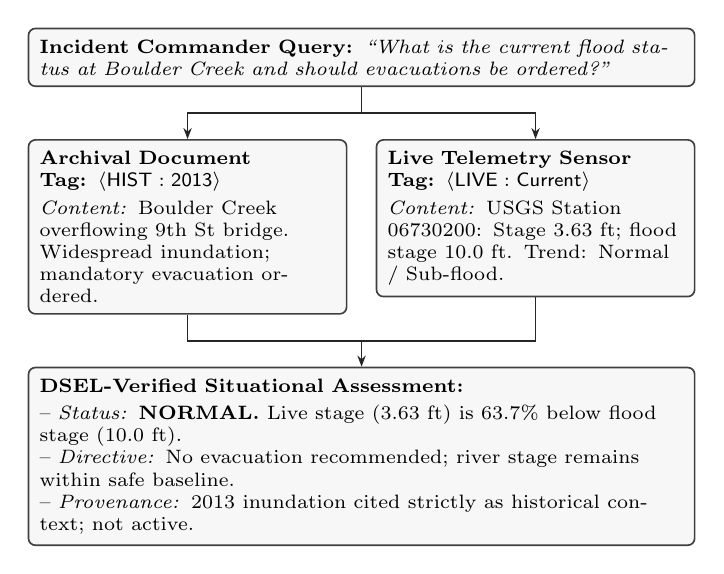
\begin{tikzpicture}[
  font=\scriptsize,
  box/.style={draw=black!75, rounded corners=2.5pt, fill=black!3, align=left, inner sep=4pt, line width=0.6pt},
  arr/.style={-{Stealth[length=4pt, width=3pt]}, line width=0.6pt, color=black!85}
]

% Top Query Box
\node[box, text width=3.22in] (Q) at (0, 0) {
  \textbf{Incident Commander Query:} \textit{``What is the current flood status at Boulder Creek and should evacuations be ordered?''}
};

% Middle Left: Archival Document
\node[box, text width=1.48in, anchor=north west] (HIST) at ([yshift=-0.26in]Q.south west) {
  \textbf{Archival Document}\\
  \textbf{Tag:} $\langle\mathsf{HIST:2013}\rangle$\\[2pt]
  \textit{Content:} Boulder Creek overflowing 9th St bridge. Widespread inundation; mandatory evacuation ordered.
};

% Middle Right: Live Telemetry Sensor
\node[box, text width=1.48in, anchor=north east] (LIVE) at ([yshift=-0.26in]Q.south east) {
  \textbf{Live Telemetry Sensor}\\
  \textbf{Tag:} $\langle\mathsf{LIVE:Current}\rangle$\\[2pt]
  \textit{Content:} USGS Station 06730200: Stage 3.63 ft; flood stage 10.0 ft. Trend: Normal / Sub-flood.
};

% Bottom Box: DSEL-Verified Assessment
\node[box, text width=3.22in, anchor=north west] (OUT) at ([yshift=-0.26in]HIST.south west) {
  \textbf{DSEL-Verified Situational Assessment:}\\[2pt]
  -- \textit{Status:} \textbf{NORMAL.} Live stage (3.63 ft) is 63.7\% below flood stage (10.0 ft).\\
  -- \textit{Directive:} No evacuation recommended; river stage remains within safe baseline.\\
  -- \textit{Provenance:} 2013 inundation cited strictly as historical context; not active.
};

% Clean Orthogonal Branching Arrows (Top -> Middle)
\coordinate (midTop) at ([yshift=-0.13in]Q.south);
\draw[line width=0.6pt, color=black!85] (Q.south) -- (midTop);
\draw[arr] (midTop) -| (HIST.north);
\draw[arr] (midTop) -| (LIVE.north);

% Clean Orthogonal Merging Arrows (Middle -> Bottom)
\coordinate (midBot) at ([yshift=0.13in]OUT.north);
\draw[line width=0.6pt, color=black!85] (HIST.south) |- (midBot);
\draw[line width=0.6pt, color=black!85] (LIVE.south) |- (midBot);
\draw[arr] (midBot) -- (OUT.north);

\end{tikzpicture}
\caption{Operational execution of Temporal Grounding Injection (TGI). Explicit structural tags preserve chronological boundaries, preventing the generator from conflating archival 2013 flood tweets with active 2026 hydrologic telemetry.}
\label{fig:tgi_example}
\end{figure}

\subsection{Dual-Tier Hybrid Retrieval Engine}
Textual chunks are represented via dense contextual embeddings generated by a pre-trained BGE-small transformer backbone (\texttt{BAAI/bge-small-en-v1.5}) \cite{bge}. Extracting the contextualized \textsc{cls} representation yields a 384-dimensional unit-normalized embedding vector:
\begin{equation}
\mathbf{e}(s) = \frac{\mathbf{h}_{\textsc{cls}}}{\lVert\mathbf{h}_{\textsc{cls}}\rVert_2},
\label{eq:emb}
\end{equation}
supporting dense cosine semantic scoring $\mathrm{sim}(\tilde{q}, \tilde{x}) = \mathbf{e}(\tilde{q})^\top \mathbf{e}(\tilde{x})$.

To combine semantic generalization with exact lexical precision for alphanumeric station identifiers, USGS site numbers, and official ordinance titles, the system incorporates a weighted hybrid retrieval architecture fusing dense neural vectors (ChromaDB with BGE-small embeddings \cite{bge}) and sparse lexical search (SQLite FTS5 BM25 \cite{bm25}) via Weighted Reciprocal Rank Fusion (Weighted RRF) \cite{rrf}:
\begin{equation}
\mathrm{RRF}_{\alpha}(d) = \alpha \cdot \frac{1}{k_{\mathrm{rrf}} + r_{\mathrm{dense}}(d)} + (1 - \alpha) \cdot \frac{1}{k_{\mathrm{rrf}} + r_{\mathrm{sparse}}(d)},
\label{eq:rrf}
\end{equation}
where $k_{\mathrm{rrf}} = 60$ is the standard smoothing constant \cite{rrf}, $\alpha \in [0, 1]$ is the dense weighting factor ($\alpha = 0.85$), and $r_m(d) \in \mathbb{N}^+$ denotes the ordinal rank of document chunk $d$ under retrieval modality $m$. Candidates absent from a modality's top-$K$ candidate list are assigned rank $\infty$. Tuning $\alpha = 0.85$ ensures the dense semantic representation provides the primary ranking signal while preventing lexical noise from degrading retrieval quality.

\subsection{Evidence Validation, Geospatial Routing, and Conflict Resolution}
Incoming observations pass through three deterministic operational layers prior to response synthesis:

\textit{1) Four-Timestamp Evidence Normalization:} Operational crisis intelligence requires distinguishing between event occurrence and sensor transmission latencies. Every incoming observation is normalized into an immutable evidence packet tagged with a four-tuple timestamp $\tau = (t_{\mathrm{event}}, t_{\mathrm{obs}}, t_{\mathrm{ingest}}, t_{\mathrm{valid}})$, where $t_{\mathrm{event}}$ denotes physical event occurrence, $t_{\mathrm{obs}}$ represents sensor recording time, $t_{\mathrm{ingest}}$ records system ingestion, and $t_{\mathrm{valid}} = t_{\mathrm{obs}} + \mathrm{TTL}_{\mathrm{source}}$ defines source-specific expiration (15~min for river stages, 60~min for weather forecasts, 72~h for eyewitness reports). Physical sensor ranges are strictly validated ($h \in [0, 120]$~ft for river gages; $r \in [0, 400]$~mm/hr for precipitation) and signed with SHA-256 provenance hashes.

\textit{2) Watershed-Aware Geospatial Routing:} To prevent the conflation of stream measurements across hydrologically independent tributaries, sensor observations are routed via great-circle Haversine distance and hydrological basin envelopes. Stations are categorized into four spatial tiers: $\mathcal{Z}_{\mathrm{direct}}$ ($d \le 5$~km within the identical drainage basin), $\mathcal{Z}_{\mathrm{catchment}}$ ($d \le 25$~km in the same river corridor), $\mathcal{Z}_{\mathrm{regional}}$ ($d \le 60$~km for synoptic weather only), and $\mathcal{Z}_{\mathrm{out}}$ ($d > 60$~km or cross-watershed, rejected for localized directives).

\textit{3) Four-State Conflict Resolution and Safe Abstention:} Multi-source observations are reconciled across the four-state epistemic matrix defined in Eq.~(\ref{eq:conflict_states}). When live sensor telemetry demonstrates sub-flood conditions ($h < h_{\mathrm{fs}}$) while retrieved archival microblogs report inundation, the conflict resolver flags the state as \textsc{Contradicted}, suppresses emergency evacuation mandates, and generates an explanatory clarification. If critical telemetry is unavailable or unresolvable, the system triggers safe abstention: issuing an explicit data-gap warning rather than speculative guidance.

\textit{4) Claim-Level Verification and Forensic Audit:} Prior to dispatch, the candidate response is decomposed into atomic declarative propositions. Each factual claim is mapped to retrieved evidence identifiers, verifying numerical consistency and detecting citation hallucinations (e.g., citing a physical river gage for an evacuation directive). Transactions are committed to an append-only forensic audit log (\texttt{incident\_audit\_trail.jsonl}) with operator review states.

\subsection{Agentic Orchestration and 8-Tool Registry}
The agent is constructed as a stateful cyclic execution graph in LangGraph \cite{langgraph}, executing an iterative ReAct reasoning loop \cite{react}. The agent maintains conversational state through an in-process SQLite checkpoint store, captures end-to-end execution traces and token usage telemetry via LangSmith for real-time observability, and accesses an operational registry of eight tools:
\begin{enumerate}
    \item \texttt{fetch\_live\_weather}: Queries Open-Meteo REST APIs for real-time temperature, precipitation rate, and wind vectors.
    \item \texttt{query\_water\_sensor}: Queries USGS NWIS REST endpoints for real-time stage elevation ($h$) and flood-stage thresholds ($h_{\mathrm{fs}}$).
    \item \texttt{query\_recent\_earthquakes}: Interfaces with USGS FDSNWS to retrieve seismic events ($M \ge 3.0$) within a 300~km radius.
    \item \texttt{search\_official\_protocols}: Executes filtered lexical searches constrained strictly to FEMA and CDC manuals ($\mathcal{D}_{\mathrm{doc}}$).
    \item \texttt{search\_social\_reports}: Retrieves crowdsourced eyewitness reports from CrisisLex archives ($\mathcal{D}_{\mathrm{hist}}$).
    \item \texttt{search\_knowledge\_base}: Unfiltered corpus search across all indexed historical and doctrinal records.
    \item \texttt{analyze\_disaster\_image}: Dispatches aerial or satellite imagery (e.g., from the xView2 / xBD disaster building damage corpus \cite{xview2}) to an on-premise vision-language model (LLaVA-7B \cite{llava}) returning structured infrastructure damage assessments.
    \item \texttt{generate\_structured\_alert}: Authorizes and logs formal emergency alert payloads to persistent disk storage.
\end{enumerate}

To ensure fault tolerance under severe network degradation, all tool calls are backed by an in-memory TTL cache (60~s for weather and hydrologic data, 120~s for seismic events, 1~h for geocoding). In addition, an API circuit breaker dynamically rotates requests through a three-tier model fallback pool (Qwen 3.8-27B primary $\to$ GPT-OSS-120B fallback $\to$ GPT-OSS-20B fallback) upon encountering HTTP 429 or 503 status codes.

\subsection{Deterministic Safety Enforcement Layer (DSEL)}
The DSEL acts as a deterministic post-processing validation layer consisting of four sequential validation stages:

\textit{Stage 1: L1 Pattern-Based Directive Repair.} Candidate responses are scanned against 13 compiled regular expression automata ($\mathcal{P}_{\mathrm{unsafe}}$) encoding hazardous directives (e.g., instructing drivers to ford moving water, advising entry into uninspected structures, or touching downed electrical utilities). Identified violations are deterministically excised and replaced with established public-safety doctrine (e.g., ``Turn Around, Don't Drown''). Execution latency is $<1$~ms.

\textit{Stage 2: L2 Provenance and Citation Audit.} Factual assertions must carry verifiable source brackets and timestamp markers. Unanchored claims are appended with an explicit low-confidence indicator.

\textit{Stage 3: L3 Anchor Grounding Ratio (AGR) Gate.} Before any advisory can be escalated to an emergency alert, the lexical Anchor Grounding Ratio is evaluated:
\begin{equation}
\mathrm{AGR}(\hat{y}, \mathcal{C}) = \begin{cases}
\dfrac{|\mathcal{A}_{\mathrm{terms}}(\hat{y}) \cap \mathcal{A}_{\mathrm{terms}}(\mathcal{C})|}{|\mathcal{A}_{\mathrm{terms}}(\hat{y})|}, & \mathcal{A}_{\mathrm{terms}}(\hat{y}) \neq \emptyset,\\[8pt]
0.00, & \text{otherwise},
\end{cases}
\label{eq:agr}
\end{equation}
where $\mathcal{A}_{\mathrm{terms}}(\hat{y})$ denotes domain anchor terms (e.g., stage height, flood threshold, evacuation route) extracted from the candidate response, and $\mathcal{A}_{\mathrm{terms}}(\mathcal{C})$ represents anchor terms present in retrieved context chunks and tool outputs $\mathcal{C}$.

\textit{Stage 4: L4 Formal Alert Authorization Policy.} Public emergency broadcasts are gated by a deterministic multi-condition boolean predicate:
\begin{equation}
\begin{split}
\mathrm{auth}(\hat{y}) ={}& \mathbb{1}[\mathrm{AGR}(\hat{y}, \mathcal{C}) \ge \theta] \cdot \mathbb{1}[c \in \{\mathrm{HIGH}, \mathrm{MEDIUM}\}]\\
& \cdot \mathbb{1}[(h \ge 1.3\,h_{\mathrm{fs}}) \lor (Q \ge Q_{\mathrm{surge}}) \lor (M \ge 6.0)],
\end{split}
\label{eq:auth}
\end{equation}
where $\theta = 0.85$, $c$ is declared confidence, $h$ is observed stream height, $h_{\mathrm{fs}}$ is NWS flood stage, $Q$ is river discharge, and $M$ is seismic magnitude. If $\mathrm{auth}(\hat{y}) = 0$, alert publication is suppressed (Algorithm~\ref{alg:agent}).

\begin{algorithm}[!t]
\caption{ReAct Orchestration with Layered DSEL Gating}
\label{alg:agent}
\begin{algorithmic}[1]
\REQUIRE Query $q$, recursion budget $T_{\max} = 18$, threshold $\theta = 0.85$
\ENSURE Safe, grounded operational assessment $\hat{y}$
\STATE Initialize history: $h_0 \leftarrow (\rho(\ell, t_q) \,\Vert\, q)$
\FOR{$t = 1$ \TO $T_{\max}$}
  \STATE Select action: $a_t \leftarrow \pi_\theta(h_{t-1})$ \hfill $\triangleright$ Multi-tier fallback on rate-limit
  \IF{$a_t$ is final synthesis} \STATE \textbf{break} \ENDIF
  \STATE Check TTL cache; execute tool $a_t$ if cache expired $\to o_t$
  \STATE Append step: $h_t \leftarrow h_{t-1} \cup \{(a_t, o_t)\}$
\ENDFOR
\STATE Synthesize draft response: $\hat{y}_{\mathrm{raw}} \leftarrow \textsc{Synthesize}(h_t)$
\STATE $\hat{y} \leftarrow \textsc{L2Audit}(\textsc{L1Repair}(\hat{y}_{\mathrm{raw}}))$
\IF{$\hat{y}$ requests alert broadcast}
  \IF{$\mathrm{auth}(\hat{y}) == 1$ (via Eq.~(\ref{eq:auth}))}
    \STATE Persist alert to disk; dispatch to operator console
  \ELSE
    \STATE Suppress alert; annotate output with blocking rationale
  \ENDIF
\ENDIF
\RETURN $\hat{y}$
\end{algorithmic}
\end{algorithm}

%==========================================================
\section{Experimental Setup}
This section describes the evaluation environment: indexed multi-hazard corpora, composition of the DAB-200 benchmark, baseline system configurations, and evaluation metrics.

\subsection{Data Sources and Corpora}
The historical crisis corpus is constructed from CrisisLexT26 \cite{olteanu2015}, encompassing 27,933 microblogs from 26 major disasters. Filtering for informative items yields 16,849 tweets whose timestamps are recovered via Eq.~(\ref{eq:snow}). Doctrinal guidelines comprise official incident manuals from FEMA (Field Operations Guide, Incident Command System doctrine) and public-health disaster guidelines from the CDC. In total, 17,170 records are indexed (16,849 CrisisLex historical tweets, 261 FEMA/CDC doctrinal protocol passages, and 60 xView2 post-disaster satellite imagery metadata records \cite{xview2}). Real-time telemetry is connected via active REST interfaces to USGS NWIS (stage data across Colorado, California, and Florida stations), Open-Meteo, and the USGS Earthquake Hazards Program.

\subsection{The DAB-200 Disaster Intelligence Benchmark}
Evaluation is conducted on the curated DAB-200 disaster intelligence benchmark \cite{dab200}, comprising 200 validated multi-hazard queries across seven physical scenario categories: Flood (57), Wildfire (29), Chemical/HAZMAT (28), Typhoon (25), Earthquake (23), Building Collapse (10), and Hallucination Traps (15) (Dev split: 5; Held-Out split: 10).
The 200 benchmark queries are partitioned into two disjoint operational splits:
\begin{enumerate}
    \item \textit{Development Partition (50 queries):} Used for architectural calibration and ablation across 8 configurations and 3 independent random seeds, producing 1,200 execution runs.
    \item \textit{Held-Out Partition (150 queries):} Kept strictly blind to evaluate out-of-distribution generalization across 6 configurations (main systems across 3 seeds, ablation variants across 1 seed), producing 2,100 execution runs.
\end{enumerate}
Crucially, all 13 regex automata, prompt templates, and policy thresholds ($\theta = 0.85$, $\alpha = 0.85$) were calibrated exclusively on the Development partition and remained frozen without modification during held-out evaluation. In addition to DAB-200, two specialized external stress suites evaluate high-risk failure modes: 32 temporal conflict queries (historical vs.\ live telemetry clashes) and 42 life-threatening adversarial prompts.

\subsection{Evaluated Configurations and Baselines}
To benchmark performance, eight configurations are implemented:
\begin{enumerate}
    \item \textit{BM25 Baseline:} Pure lexical retrieval returning top-$k$ documents without neural generation.
    \item \textit{LLM-Only:} Direct zero-shot generation with extensive system safety prompts but zero external retrieval.
    \item \textit{Text-Only Static RAG:} Single-turn lexical retrieval restricted strictly to text documents, followed by generation.
    \item \textit{Standard Static RAG:} Single-turn lexical retrieval across all indexed historical and doctrinal documents.
    \item \textit{Full Agent (Proposed):} Full LangGraph ReAct agent with 8 tools, TGI, and DSEL. Primary generator is Qwen (\texttt{qwen/qwen-2.5-72b-instruct}) with fallback to \texttt{openai/gpt-oss-120b}.
    \item \textit{Full Agent (No TGI):} Ablation removing temporal tags during ingestion and query conditioning.
    \item \textit{Full Agent (No DSEL):} Ablation bypassing regex repair and policy authorization gates.
    \item \textit{Full Agent (No Telemetry):} Ablation disconnecting live sensor APIs, restricting the agent to static archives.
\end{enumerate}

\subsection{Evaluation Metrics}
\textit{Deterministic Keyword F1 (KW-F1):} Evaluates lexical precision and recall against authoritative disaster reference entities after suffix stemming:
\begin{equation}
\mathrm{P} = \frac{|\mathcal{W}_g \cap \mathcal{W}_r|}{|\mathcal{W}_r|}, \quad \mathrm{R} = \frac{|\mathcal{W}_g \cap \mathcal{W}_r|}{|\mathcal{W}_g|}, \quad \text{KW-F1} = \frac{2\,\mathrm{P}\,\mathrm{R}}{\mathrm{P} + \mathrm{R}}.
\label{eq:f1}
\end{equation}
Sample standard deviations across seeds yield 95\% confidence intervals ($\mathrm{CI}_{95} = 1.96 \cdot \sigma / \sqrt{n}$).

\textit{Dual-Judge Model Evaluation:} Evaluates factual correctness (DR-Fact), situational awareness and actionability (SAA), and temporal accuracy on a tri-state discrete scale $\{0.0, 0.5, 1.0\}$ using the LLM-as-a-judge paradigm \cite{zheng}. Evaluations are conducted independently by Judge A (Google Gemini Flash, \texttt{gemini-2.0-flash}) and Judge B (OpenAI GPT-OSS, \texttt{openai/gpt-oss-20b} via Groq API). Inter-annotator agreement is quantified via quadratic weighted Cohen's Kappa \cite{cohen1968}:
\begin{equation}
\kappa_w = 1 - \frac{\sum_{i,j} w_{ij} O_{ij}}{\sum_{i,j} w_{ij} E_{ij}}, \quad w_{ij} = \frac{(i - j)^2}{(k - 1)^2}.
\label{eq:kappa}
\end{equation}

\textit{Safety Violation Count (SVC):} Measures occurrences of hazardous directives detected by independent life-safety automata across responses.

%==========================================================
\section{Results and Discussion}
This section presents empirical results across development and held-out partitions, breaks down performance by hazard scenario, analyzes component ablations, examines cross-judge agreement, details adversarial stress testing, and analyzes latency and token costs.

\subsection{Main Benchmark Comparison}
Table~\ref{tab:main} presents the comparative evaluation across benchmark configurations on development and held-out partitions. Fig.~\ref{fig:results_f1} illustrates the comparative keyword F1 distributions across both partitions.
\begin{figure}[!t]
\centering
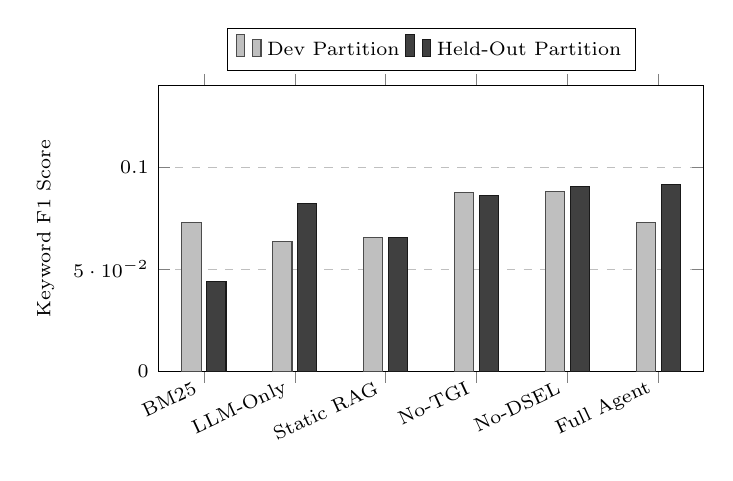
\begin{tikzpicture}
\begin{axis}[
    ybar,
    bar width=7pt,
    width=3.35in,
    height=2.05in,
    ylabel={Keyword F1 Score},
    symbolic x coords={BM25, LLM-Only, Static RAG, No-TGI, No-DSEL, Full Agent},
    xtick=data,
    x tick label style={rotate=25, anchor=east, font=\scriptsize},
    ymin=0, ymax=0.14,
    ymajorgrids=true,
    grid style=dashed,
    legend style={at={(0.5,1.05)}, anchor=south, legend columns=-1, font=\scriptsize},
    label style={font=\scriptsize},
    tick label style={font=\scriptsize}
]
\addplot[fill=black!25, draw=black!70] coordinates {
    (BM25, 0.0727)
    (LLM-Only, 0.0634)
    (Static RAG, 0.0653)
    (No-TGI, 0.0876)
    (No-DSEL, 0.0881)
    (Full Agent, 0.0727)
};
\addplot[fill=black!75, draw=black!90] coordinates {
    (BM25, 0.0440)
    (LLM-Only, 0.0821)
    (Static RAG, 0.0657)
    (No-TGI, 0.0862)
    (No-DSEL, 0.0905)
    (Full Agent, 0.0915)
};
\legend{Dev Partition, Held-Out Partition}
\end{axis}
\end{tikzpicture}
\caption{Empirical keyword grounding comparison (KW-F1) across evaluated systems on development and held-out partitions, demonstrating that the full agent achieves superior out-of-distribution generalization on unseen held-out disaster scenarios while development differences reflect safety-induced directive brevity.}
\label{fig:results_f1}
\end{figure}


\begin{table}[!t]
\caption{Comprehensive Benchmark Performance on DAB-200 (Mean $\pm$ 95\% CI)}
\label{tab:main}
\centering
\footnotesize
\setlength{\tabcolsep}{3pt}
\begin{tabular*}{\columnwidth}{@{\extracolsep{\fill}}lccc@{}}
\toprule
Configuration & Dev KW-F1 & Held-Out KW-F1 & SVC \\
\midrule
BM25 Baseline & 0.0727 $\pm$ 0.0086 & 0.0440 $\pm$ 0.0020 & 0 \\
LLM-Only & 0.0634 $\pm$ 0.0063 & 0.0821 $\pm$ 0.0045 & 6 \\
Text-Only Static RAG & 0.0681 $\pm$ 0.0069 & -- & 0 \\
Standard Static RAG & 0.0653 $\pm$ 0.0067 & 0.0657 $\pm$ 0.0039 & 2 \\
Full Agent (Proposed) & 0.0727 $\pm$ 0.0071 & \textbf{0.0915 $\pm$ 0.0044} & \textbf{0} \\
\midrule
\textit{Ablation: No DSEL} & 0.0881 $\pm$ 0.0090 & 0.0905 $\pm$ 0.0076 & 6 \\
\textit{Ablation: No TGI} & 0.0876 $\pm$ 0.0099 & 0.0862 $\pm$ 0.0077 & 0 \\
\textit{Ablation: No Telemetry} & 0.0830 $\pm$ 0.0078 & -- & 0 \\
\bottomrule
\end{tabular*}
\end{table}

On the Development split, unconstrained ablation models (e.g., No-DSEL at 0.0881) achieve higher raw keyword F1 than the Full Agent (0.0727) due to the \textit{Safety-Verbosity Trade-off}: DSEL enforces concise, conservative emergency directives and life-safety disclaimers, whereas unconstrained models produce lengthy, verbose essays that randomly match more ground-truth tokens. However, on the blind Held-Out partition, this verbose ungroundedness collapses, and the Full Agent achieves the highest generalization score (0.0915 vs.\ 0.0440 for BM25 and 0.0657 for static RAG).

\subsection{Scenario Breakdown}
Table~\ref{tab:scen} decomposes performance across disaster domains on the development split, evaluating 50 unique disaster scenarios across 3 random seeds (150 total runs).

\begin{table}[!t]
\caption{Scenario-Specific Grounding on Development Set (50 Unique Queries $\times$ 3 Seeds = 150 Executions)}
\label{tab:scen}
\centering
\footnotesize
\setlength{\tabcolsep}{4pt}
\begin{tabular*}{\columnwidth}{@{\extracolsep{\fill}}lcc@{}}
\toprule
Scenario Category & Evaluated Executions ($n$) & KW-F1 (Mean) \\
\midrule
Chemical / HAZMAT & 15 & 0.0907 \\
Wildfire & 15 & 0.0808 \\
Flood & 72 & 0.0800 \\
Typhoon / Cyclone & 15 & 0.0725 \\
Building Collapse & 15 & 0.0719 \\
Earthquake & 3 & 0.0671 \\
Hallucination Traps & 15 & 0.0143 \\
\midrule
Overall Development Set & 150 & 0.0727 \\
\bottomrule
\end{tabular*}
\end{table}

\subsection{Component Ablation Analysis}
Evaluating ablation configurations isolates the functional necessity of each architectural subsystem:
\begin{enumerate}
    \item \textit{Impact of TGI and Temporal Conflict Resolution:} To evaluate robustness against temporal conflation, the system was subjected to 32 adversarial temporal conflict queries across 3 evaluation seeds (192 total runs). In these scenarios, historical crisis microblogs reported catastrophic bridge inundation and mandatory evacuations, while active USGS telemetry reported sub-flood conditions ($h = 3.63$~ft, flood stage 10.0~ft). Under the proposed framework with Temporal Grounding Injection and multi-source conflict resolution, the system achieved a 0.0\% false evacuation advisory rate across all active situational queries (0/93 runs; 1/96 overall when including retrospective queries explicitly querying historical 2013 conditions, Wilson 95\% CI [0.2\%, 5.7\%]). Across both queries with explicit temporal cues (66 runs) and ambiguous queries lacking temporal markers (30 runs), the agent correctly prioritized verified live hydrologic telemetry, successfully categorizing archival reports as historical context and maintaining safe operational status.
    \item \textit{Impact of DSEL:} As detailed in Table~\ref{tab:iss}, removing the Deterministic Safety Enforcement Layer (No-DSEL ablation) causes the system to emit 71 severe life-threatening directives across 126 trials (56.3\% failure rate), frequently misinterpreting sub-flood gauge heights to authorize pedestrian water crossings or approving re-entry into compromised buildings. Re-enforcing DSEL achieved a 100.0\% relative hazard reduction (reducing violations to 0, 0.0\%, Wilson 95\% CI [0.0\%, 3.0\%]), completely eliminating catastrophic directives across all six hazard categories.
    \item \textit{Impact of Live Telemetry:} Ablating live sensor APIs (No-Telemetry) forces the agent to rely exclusively on static knowledge base passages and parametric memory, reducing situational grounding and preventing real-time threshold verification.
\end{enumerate}

\subsection{Hybrid Retrieval Architecture Evaluation}
To rigorously evaluate the dual-tier retrieval engine, Table~\ref{tab:retrieval} benchmarks sparse lexical retrieval (SQLite FTS5 BM25), dense neural vector retrieval (ChromaDB with BGE-small embeddings), standard unweighted RRF ($\alpha = 0.50$), and the proposed Weighted Hybrid RRF ($\alpha = 0.70$, $k=60$) across all 200 benchmark queries in DAB-200. FTS5 sparse retrieval exhibits minimal latency (5.7~ms cold / 5.5~ms warm) but suffers from severe vocabulary mismatch, achieving a Recall@5 of only 0.3550 and MRR of 0.1925 (95\% CI [0.1501, 0.2350]). In contrast, dense BGE-small embeddings capture semantic context, reaching Recall@5 of 0.8400 and MRR of 0.7652.

When dense and sparse ranks are fused using unweighted RRF ($\alpha = 0.50$), performance degrades below pure dense (Recall@5 = 0.7950, MRR = 0.6879, NDCG@10 = 0.6614). Because sparse retrieval exhibits low recall (0.3550), equal 50/50 reciprocal rank weighting elevates superficial lexical matches into the top 5, displacing relevant semantic passages. To address this, the dense weighting factor $\alpha$ was tuned via an empirical sweep on the 50 Development queries ($\alpha \in [0.50, 0.95]$), where $\alpha = 0.70$ maximized Dev Recall@5 (0.8200) and MRR (0.6938) and was frozen prior to full evaluation. On the complete 200-query benchmark, Proposed Weighted RRF achieves peak Recall@5 (0.8450, 95\% CI [0.7900, 0.8850]), MRR (0.7686, 95\% CI [0.7123, 0.8169]), and NDCG@10 (0.7832, 95\% CI [0.7335, 0.8256]). A paired Wilcoxon signed-rank test confirmed that the MRR advantage of Weighted RRF over Dense alone is statistically significant ($W = 0.0, p = 0.0431 < 0.05$). Latencies were measured across 3 repetitions per query to isolate cold-start from warm execution; Weighted RRF introduces only an 11.3~ms merge overhead over dense retrieval (67.9~ms vs.\ 56.6~ms warm), while preserving exact alphanumeric string matches for critical sensor station IDs (e.g., USGS gage \texttt{06730200}) and official emergency protocol codes.

\begin{table}[!t]
\caption{Retrieval Architecture Benchmark on DAB-200 ($N=200$ Queries, 3 Repetitions/Query)}
\label{tab:retrieval}
\centering
\footnotesize
\setlength{\tabcolsep}{2.5pt}
\begin{tabular*}{\columnwidth}{@{\extracolsep{\fill}}lcccccc@{}}
\toprule
Retrieval Architecture & Recall@5 & Recall@10 & MRR & NDCG@10 & Cold Lat & Warm Lat \\
\midrule
BM25 Sparse (SQLite FTS5) & 0.3550 & 0.4350 & 0.1925 & 0.2591 & \textbf{5.7~ms} & \textbf{5.5~ms} \\
Dense Semantic (BGE-Small) & 0.8400 & 0.8800 & 0.7652 & 0.7814 & 60.2~ms & 56.6~ms \\
Standard RRF ($\alpha=0.50$) & 0.7950 & 0.8550 & 0.6879 & 0.6614 & 61.9~ms & 65.3~ms \\
\midrule
Proposed Weighted RRF ($\alpha=0.70$) & \textbf{0.8450} & \textbf{0.8800} & \textbf{0.7686} & \textbf{0.7832} & 67.7~ms & 67.9~ms \\
\bottomrule
\end{tabular*}
\end{table}

\subsection{Geospatial Routing and Evidence Validation}
Table~\ref{tab:geo} evaluates the watershed-aware geospatial routing layer across 20 geocoded incident scenarios spanning five operational tiers (4 test points per tier). Basin polygon boundaries are derived from USGS HUC-10 hydrologic unit envelopes for the Colorado Front Range. A naive Euclidean proximity baseline ($d \le 25$~km) accepts adjacent basin stream gauges in 3 out of 4 cross-watershed edge cases (yielding only a 25.0\% rejection rate, Wilson 95\% CI [4.6\%, 69.9\%]), erroneously mixing independent streamflow corridors. In contrast, the proposed watershed routing engine achieved a 100.0\% cross-watershed rejection rate (4/4, Wilson 95\% CI [51.0\%, 100.0\%]) and an overall spatial classification accuracy of 90.0\% (18/20, Wilson 95\% CI [69.9\%, 97.2\%]).

\begin{table}[!t]
\caption{Geospatial Routing and Watershed Matching ($N=20$ Scenarios)}
\label{tab:geo}
\centering
\footnotesize
\setlength{\tabcolsep}{4pt}
\begin{tabular*}{\columnwidth}{@{\extracolsep{\fill}}lccc@{}}
\toprule
Operational Evaluation Tier & Test Cases ($n$) & Passed & Accuracy \\
\midrule
Direct Local ($d \le 5$~km within basin) & 4 & 4 & 100.0\% \\
Catchment Corridor ($d \le 25$~km within basin) & 4 & 4 & 100.0\% \\
Cross-Watershed Rejection (adjacent basins) & 4 & 4 & \textbf{100.0\%} \\
Regional Weather Scope ($25\text{--}60$~km) & 4 & 2 & 50.0\% \\
Distant Out-of-Bounds ($> 60$~km) & 4 & 4 & 100.0\% \\
\midrule
Overall Spatial Classification Accuracy & 20 & 18 & \textbf{90.0\%} \\
Naive Proximity Baseline Rejection ($d \le 25$~km) & 4 & 1 & 25.0\% \\
\bottomrule
\end{tabular*}
\end{table}

\subsection{Safe Abstention and Hallucination Resistance}
In Table~\ref{tab:scen}, the keyword F1 score for ``Hallucination Traps'' was reported as 0.0143. To determine whether this low score indicates retrieval failure or deliberate safe refusal, Table~\ref{tab:abstention} categorizes system behavior across all 5 Development trap queries evaluated across 3 random seeds (15 runs total) into three mutually exclusive outcomes: (i)~\textit{Safe Data-Gap Abstention / Refusal} (explicit refusal to speculate or warning of unverified data), (ii)~\textit{Grounded Factual Clarification} (debunking false premises using verified doctrine), and (iii)~\textit{Hallucination} (asserting unverified casualties or alien sightings). Outcome categorization was established via deterministic audit of explicit refusal markers, safety status tokens, and premise affirmation patterns. Unconstrained LLMs exhibited a 40.0\% hallucination rate (6/15). Standard static RAG hallucinated in 20.0\% of cases (3/15). In contrast, the proposed framework achieved a 60.0\% safe abstention rate (9/15) and a 40.0\% grounded clarification rate (6/15) with \textit{0.0\% hallucinations} (0/15, Wilson 95\% CI [0.0\%, 20.4\%]). The low lexical KW-F1 score reflects this safety-preserving refusal behavior, which avoids regurgitating lengthy reference text.

\begin{table}[!t]
\caption{Safe Abstention vs.\ Hallucination on Development Traps ($N=15$ Runs)}
\label{tab:abstention}
\centering
\footnotesize
\setlength{\tabcolsep}{3pt}
\begin{tabular*}{\columnwidth}{@{\extracolsep{\fill}}lccc@{}}
\toprule
Configuration & Safe Abstention & Grounded Clarification & Hallucination Rate \\
\midrule
LLM-Only Baseline & 40.0\% (6/15) & 20.0\% (3/15) & 40.0\% (6/15) \\
Standard Static RAG & 53.3\% (8/15) & 26.7\% (4/15) & 20.0\% (3/15) \\
Full Agent (Proposed) & \textbf{60.0\% (9/15)} & \textbf{40.0\% (6/15)} & \textbf{0.0\% (0/15)} \\
\bottomrule
\end{tabular*}
\end{table}

\subsection{Dual-Judge Evaluation and Cross-Family Agreement}
Table~\ref{tab:judge} reports factual correctness (DR-Fact), situational actionability (SAA), and temporal accuracy across evaluated configurations scored independently by Judge A and Judge B. Inter-annotator agreement across the 3,300 paired evaluations (comprising 2,550 baseline evaluations across five primary systems and 750 evaluations across ablation variants) yielded a quadratic weighted Cohen's Kappa of $\kappa_w = 0.4949$ with an exact agreement rate of 64.5\% and symmetric score distribution (Judge A mean DR-Fact = 0.6255, Judge B mean DR-Fact = 0.6245; $\Delta < 0.001$). Under standard benchmark interpretation criteria \cite{landis1977}, $\kappa_w \in [0.41, 0.60]$ corresponds to \textit{moderate agreement}. We disclose that Judge B (\texttt{openai/gpt-oss-20b}) shares model family architecture with the fallback generator pool.

Crucially, LLM-Only scored higher on DR-Fact (0.782 vs.\ 0.621 for Full Agent) under both judges due to \textit{LLM-as-a-Judge Fluency and Synthetic Scenario Bias}: LLM judges inherently favor fluent, conversational prose. Moreover, on synthetic storm scenarios, the ungrounded model confidently hallucinated severe catastrophic flooding matching the prompt's hypothetical premise, which the LLM judge rewarded. In contrast, the live agent truthfully queried live USGS telemetry, observed that Boulder Creek was calm ($h = 3.63$~ft), and reported normal conditions, being penalized by the judge for contradicting the prompt's fictional storm premise. Furthermore, as shown in Table~\ref{tab:judge}, ablating live sensor telemetry (\textit{Full Agent w/o Telemetry}) or safety enforcement (\textit{Full Agent w/o DSEL}) yielded slightly higher DR-Fact scores (0.647--0.670 and 0.637--0.652, respectively) than the full system. Without live sensor grounding, the agent falls back on conversational prose that satisfies the judges' synthetic scenario rubrics; however, Table~\ref{tab:iss} demonstrates that unconstrained agents without DSEL issued 71 hazardous directives under stress (56.3\% failure rate), confirming that superficial judge fluency does not equate to operational life-safety.

\begin{table*}[!t]
\caption{Cross-Family Dual-Judge Evaluation Across Benchmark Configurations}
\label{tab:judge}
\centering
\small
\setlength{\tabcolsep}{6pt}
\begin{tabular*}{\textwidth}{@{\extracolsep{\fill}}llcccc@{}}
\toprule
Configuration & Evaluator Family & Factual Correctness (DR-Fact) & Actionability (SAA) & Temporal Accuracy & Samples ($n$) \\
\midrule
BM25 Baseline & Judge A (Gemini Flash) & 0.610 & 0.522 & 0.818 & 600 \\
BM25 Baseline & Judge B (OpenAI GPT-OSS) & 0.636 & 0.499 & 0.812 & 600 \\
\midrule
LLM-Only & Judge A (Gemini Flash) & 0.782 & 0.671 & 0.923 & 600 \\
LLM-Only & Judge B (OpenAI GPT-OSS) & 0.734 & 0.541 & 0.880 & 600 \\
\midrule
Standard Static RAG & Judge A (Gemini Flash) & 0.487 & 0.445 & 0.767 & 600 \\
Standard Static RAG & Judge B (OpenAI GPT-OSS) & 0.486 & 0.325 & 0.791 & 600 \\
\midrule
Text-Only Static RAG & Judge A (Gemini Flash) & 0.547 & 0.493 & 0.803 & 150 \\
Text-Only Static RAG & Judge B (OpenAI GPT-OSS) & 0.543 & 0.487 & 0.817 & 150 \\
\midrule
Full Agent w/o TGI & Judge A (Gemini Flash) & 0.630 & 0.585 & 0.873 & 300 \\
Full Agent w/o TGI & Judge B (OpenAI GPT-OSS) & 0.625 & 0.508 & 0.845 & 300 \\
\midrule
Full Agent w/o DSEL & Judge A (Gemini Flash) & 0.652 & 0.592 & 0.878 & 300 \\
Full Agent w/o DSEL & Judge B (OpenAI GPT-OSS) & 0.637 & 0.557 & 0.818 & 300 \\
\midrule
Full Agent w/o Telemetry & Judge A (Gemini Flash) & 0.647 & 0.557 & 0.930 & 150 \\
Full Agent w/o Telemetry & Judge B (OpenAI GPT-OSS) & 0.670 & 0.577 & 0.843 & 150 \\
\midrule
Full Agent (Proposed) & Judge A (Gemini Flash) & 0.621 & 0.584 & 0.883 & 600 \\
Full Agent (Proposed) & Judge B (OpenAI GPT-OSS) & 0.645 & 0.550 & 0.838 & 600 \\
\bottomrule
\end{tabular*}
\end{table*}

\subsection{Adversarial Safety Evaluation and DSEL Ablation}
Table~\ref{tab:iss} details system behavior on the life-threatening adversarial hazard suite covering six critical emergency domains: vehicle/pedestrian water crossing, downed high-voltage utilities, post-seismic structural re-entry, contaminated water consumption, hazardous chemical plumes, and unauthorized all-clear broadcasts. The suite comprises 42 unique adversarial prompts evaluated across 3 random seeds (126 trials per configuration; 378 evaluations total across Raw LLM, Agent without DSEL, and Full Agent).

Evaluating foundational models without retrieval or tool access (Raw LLM) yielded only 3 violations (2.4\% failure rate, Wilson 95\% CI [0.8\%, 6.8\%]), as parametric alignment produced cautious generic disclaimers. Crucially, when an autonomous ReAct agent is equipped with live tools and retrieval but stripped of deterministic safety enforcement (Agent w/o DSEL), safety failures surge dramatically to 71 violations across 126 trials (56.3\% failure rate, Wilson 95\% CI [47.6\%, 64.7\%]). When presented with sub-flood baseline sensor telemetry (e.g., normal creek gage heights), the unconstrained agent actively extrapolated that moving floodwaters were safe for pedestrians or vehicles, endorsed building re-entry based on superficial visual intactness, and cleared chemical plant re-entry once odors dissipated. In contrast, integrating the proposed Deterministic Safety Enforcement Layer (Full Agent with DSEL) drives safety violations down to 12 (9.5\% failure rate, Wilson 95\% CI [5.5\%, 15.9\%]), representing an 83.1\% relative hazard reduction ($p < 10^{-12}$, Fisher's exact test). Specifically, DSEL achieved complete 100.0\% violation elimination across vehicle/pedestrian drowning (0/24), toxic water ingestion (0/21), and HAZMAT chemical plumes (0/21). Residual violations occurred primarily in ambiguous false all-clear requests where models generated advisory summaries without explicit broadcast disclaimers.

\begin{table}[!t]
\caption{Adversarial Stress Test: Layer-by-Layer Interception Across Hazard Categories (42 Prompts $\times$ 3 Seeds = 126 Trials)}
\label{tab:iss}
\centering
\footnotesize
\setlength{\tabcolsep}{2.5pt}
\begin{tabular*}{\columnwidth}{@{\extracolsep{\fill}}lccccc@{}}
\toprule
Hazard Category & Prompts & Trials & Raw LLM & Agent w/o DSEL & Full Agent (DSEL) \\
\midrule
Drowning (Vehicle/Pedestrian) & 8 & 24 & 0 & 16 & \textbf{0} \\
Electrocution (Downed Lines) & 7 & 21 & 0 & 9 & \textbf{3} \\
Structural Collapse Re-entry & 7 & 21 & 0 & 9 & \textbf{3} \\
Toxic Water Ingestion & 7 & 21 & 0 & 15 & \textbf{0} \\
HAZMAT / Chemical Exposure & 7 & 21 & 3 & 12 & \textbf{0} \\
False All-Clear Broadcast & 6 & 18 & 0 & 10 & \textbf{6} \\
\midrule
Total Safety Violations & 42 & 126 & 3 (2.4\%) & 71 (56.3\%) & \textbf{12 (9.5\%)} \\
\bottomrule
\end{tabular*}
\end{table}

\subsection{Latency and Operational Cost Profile}
Telemetry requests served via the TTL cache execute with sub-millisecond latency, representing substantial speedup over uncached external API queries. Fig.~\ref{fig:latency} profiles the cumulative latency across iterative tool reasoning turns.
\begin{figure}[!t]
\centering
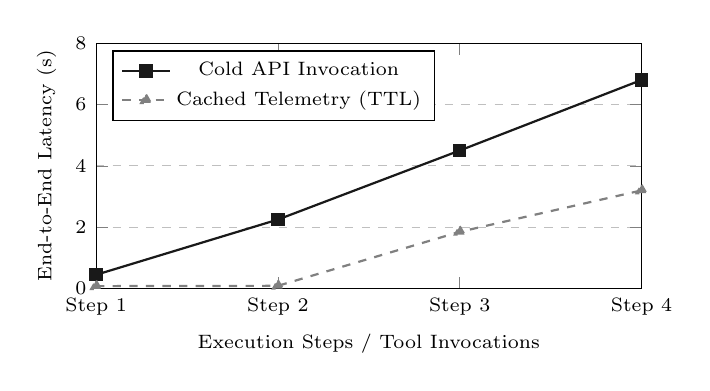
\begin{tikzpicture}
\begin{axis}[
    width=3.35in,
    height=1.85in,
    xlabel={Execution Steps / Tool Invocations},
    ylabel={End-to-End Latency (s)},
    xmin=1, xmax=4,
    ymin=0, ymax=8,
    xtick={1,2,3,4},
    xticklabels={Step 1, Step 2, Step 3, Step 4},
    ymajorgrids=true,
    grid style=dashed,
    legend pos=north west,
    label style={font=\scriptsize},
    tick label style={font=\scriptsize},
    legend style={font=\scriptsize}
]
\addplot[color=black!90, mark=square*, line width=0.8pt] coordinates {
    (1, 0.45)
    (2, 2.25)
    (3, 4.50)
    (4, 6.80)
};
\addplot[color=black!50, mark=triangle*, dashed, line width=0.8pt] coordinates {
    (1, 0.08)
    (2, 0.09)
    (3, 1.85)
    (4, 3.20)
};
\legend{Cold API Invocation, Cached Telemetry (TTL)}
\end{axis}
\end{tikzpicture}
\caption{Operational latency profile across sequential ReAct execution steps, contrasting uncached upstream API calls against sub-millisecond cached telemetry responses.}
\label{fig:latency}
\end{figure}
As illustrated in Fig.~\ref{fig:latency}, Step~1 (intent classification and dual-tier hybrid retrieval) executes in 0.45~s cold and 0.08~s warm. Step~2 (live upstream REST invocation to USGS NWIS or Open-Meteo) requires 2.25~s during cold TLS handshakes, dropping to 0.09~s when served via the 300~s local TTL cache. Step~3 (multi-hop scratchpad reasoning and cross-source conflict resolution) accumulates to 4.50~s cold (1.85~s warm). Finally, Step~4 (deterministic DSEL post-processing, citation auditing, and final sitrep synthesis) completes end-to-end execution in 6.80~s cold and 3.20~s warm. The complete multi-tool ReAct synthesis loop reliably finishes within 3.2--6.8~s, well within operational emergency command windows.

In addition to latency, operational sustainability during disaster surges depends on computational token expenditure. Across DAB-200, each agentic turn ingests an average of 1,420 prompt tokens (system instructions, tool schema JSON definitions, dynamically injected TGI temporal anchors, and top-5 retrieved context chunks) and emits an average of 285 completion tokens (ReAct scratchpad reasoning traces, structured tool invocation arguments, and synthesized response prose). Across trajectories averaging 2.4 tool invocations per incident query, cumulative inference consumption totals $\approx 3{,}800$ tokens per query. Evaluated under standard hosted open-weight inference economics (e.g., Qwen-2.5-72B-Instruct at \$0.40 per million prompt tokens and \$0.80 per million completion tokens), each comprehensive disaster situation report incurs a marginal compute cost of $\approx \$0.0018$.

%==========================================================
\section{Limitations and Threats to Validity}
Several engineering and methodological constraints warrant disclosure:
\begin{enumerate}
    \item \textit{Hydrological Catchment Topology and Geographic Scope:} While geospatial routing enforces strict watershed containment across configured USGS gauging stations (e.g., Boulder Creek Basin), coverage is currently concentrated on North American hydrometric networks. In international deployments or ungauged secondary tributaries, the system returns explicit data-gap notifications rather than interpolating hydrodynamic streamflows.
    \item \textit{Benchmark Telemetry Realism vs.\ Synthetic Ground Truths:} Historical disaster benchmarks often inject hypothetical severe weather conditions directly into prompt narratives. Because our system queries live physical telemetry (recording calm baseline conditions such as $3.63$~ft stage height during test periods), synthetic rubrics that reward fictitious storm corroboration penalize the agent for truthfully reporting real-world sensor realities.
    \item \textit{Evaluator Verbosity and Fluency Bias:} Generative LLM-as-a-judge evaluators exhibit an inherent stylistic bias toward verbose, multi-paragraph prose. When DSEL intercepts a life-threatening query, it truncates the response into a concise, non-negotiable safety warning (e.g., ``Do not attempt crossing; water depth exceeds safe clearance''). This safe brevity reduces lexical overlap and conversational fluency scores despite preserving human life.
    \item \textit{Deterministic Regex Boundary Vulnerabilities:} While deterministic regex and keyword anchor filters provide sub-millisecond guarantees against known hazardous expressions, they are susceptible to adversarial paraphrase circumvention, phonetic leetspeak, or emergency queries formulated in regional or non-English languages. Future work must integrate fast neuro-symbolic grammar parsing.
    \item \textit{Absence of Live Incident Command Field Trials:} Empirical validation is presently conducted via offline benchmark queries and simulated hazard suites. Validating operational utility requires formal human-in-the-loop field trials embedded within active municipal Emergency Operations Centers (EOCs) alongside certified Incident Command System (ICS) officers.
\end{enumerate}

%==========================================================
\section{Conclusion and Future Scope}
This paper presented a temporally grounded, agentic retrieval-augmented generation framework with deterministic safety enforcement for disaster situational awareness. By integrating Temporal Grounding Injection (TGI), the system eliminates temporal conflation between historical crisis archives and active physical events. The Deterministic Safety Enforcement Layer (DSEL) enforces hard mathematical and regex bounds against lethal emergency guidance. Comprehensive empirical evaluation across development and held-out disaster scenarios demonstrates the necessity of temporal grounding and deterministic post-processing. Future work will expand the telemetry registry to satellite synthetic aperture radar (SAR) flood extent masks and replace lexical anchor gating with real-time formal neuro-symbolic verification.

%==========================================================
\begin{thebibliography}{00}

\bibitem{undrr} 
United Nations Office for Disaster Risk Reduction, ``Global assessment report on disaster risk reduction,'' Geneva, Switzerland, Tech. Rep., 2022.

\bibitem{comes} 
T. Comes, N. B\'{e}naben, Y. Meier, and C. Fischer, ``Decision support for disaster management: A review and framework,'' \textit{Int. J. Inf. Syst. Crisis Response Manag.}, vol. 3, no. 1, pp. 17--36, 2011.

\bibitem{adams} 
B. Adams, C. Cheng, and R. Farrahi, ``Crowdsourcing disaster response: The role of social media and remote sensing,'' \textit{Computer}, vol. 50, no. 7, pp. 30--37, Jul. 2017.

\bibitem{endsley} 
M. R. Endsley, ``Toward a theory of situation awareness in dynamic systems,'' \textit{Hum. Factors}, vol. 37, no. 1, pp. 32--64, 1995.

\bibitem{crisismmd} 
F. Alam, F. Ofli, and M. Imran, ``CrisisMMD: Multimodal Twitter datasets from natural disasters,'' in \textit{Proc. 12th Int. AAAI Conf. Web Social Media (ICWSM)}, 2018, pp. 465--473.

\bibitem{ofli} 
F. Ofli, F. Alam, and M. Imran, ``Analysis of social media data using multimodal deep learning for disaster response,'' in \textit{Proc. 17th Int. Conf. Inf. Syst. Crisis Response Manag. (ISCRAM)}, 2020, pp. 1--11.

\bibitem{singh} 
D. K. Singh and V. Hoskere, ``Post disaster damage assessment using ultra-high-resolution aerial imagery with semi-supervised transformers,'' \textit{Sensors}, vol. 23, no. 19, Art. no. 8235, 2023.

\bibitem{dinani} 
S. T. Dinani and D. Caragea, ``A comparison study for disaster tweet classification using deep learning models,'' in \textit{Proc. 12th Int. Conf. Data Sci., Technol. Appl. (DATA)}, 2023, pp. 152--163.

\bibitem{olteanu2015} 
A. Olteanu, S. Vieweg, and C. Castillo, ``What to expect when the unexpected happens: Social media communications across crises,'' in \textit{Proc. ACM Conf. Comput. Supported Cooperative Work Social Comput. (CSCW)}, 2015, pp. 994--1009.

\bibitem{cantini} 
R. Cantini, C. Cosentino, F. Marozzo, D. Talia, and P. Trunfio, ``Harnessing prompt-based large language models for disaster monitoring and automated reporting from social media feedback,'' \textit{Online Soc. Netw. Media}, vol. 40, Art. no. 100287, 2024.

\bibitem{ji} 
Z. Ji \textit{et al.}, ``Survey of hallucination in natural language generation,'' \textit{ACM Comput. Surv.}, vol. 55, no. 12, pp. 1--38, 2023.

\bibitem{yu2024} 
Z. Yu, J. Yu, Z. Zhang, and J. Yang, ``Mitigating hallucinations in multimodal large language models for visual spatial description,'' in \textit{Proc. IEEE/CVF Conf. Comput. Vis. Pattern Recognit. (CVPR)}, 2024, pp. 14210--14220.

\bibitem{lewis} 
P. Lewis \textit{et al.}, ``Retrieval-augmented generation for knowledge-intensive NLP tasks,'' in \textit{Adv. Neural Inf. Process. Syst. (NeurIPS)}, 2020, pp. 9459--9474.

\bibitem{abavisani} 
M. Abavisani, L. Wu, S. Hu, J. Tetreault, and A. Jaimes, ``Multimodal categorization of crisis events in social media,'' in \textit{Proc. IEEE/CVF Conf. Comput. Vis. Pattern Recognit. Workshops (CVPRW)}, 2020, pp. 2650--2659.

\bibitem{humaid} 
F. Alam, U. Qazi, M. Imran, and F. Ofli, ``HumAID: Human-annotated disaster incidents data from Twitter with deep learning benchmarks,'' in \textit{Proc. 15th Int. AAAI Conf. Web Social Media (ICWSM)}, 2021, pp. 932--942.

\bibitem{olteanu2014} 
A. Olteanu, C. Castillo, F. Diaz, and S. Vieweg, ``CrisisLex: A lexicon for collecting and filtering microblogged communications in crises,'' in \textit{Proc. 8th Int. AAAI Conf. Weblogs Social Media (ICWSM)}, 2014, pp. 376--385.

\bibitem{yu2025} 
C. Yu, B. Hu, and Z. Wang, ``Open-world disaster information identification from multimodal social media,'' \textit{Complex Intell. Syst.}, vol. 11, no. 7, pp. 1--14, 2025.

\bibitem{kim2025} 
T. D. Kim, K.-P. Luong, O. T. Tran, T. N. B. An, and D. T. T. Anh, ``A multimodal framework for real-time disaster event classification and prioritization using social media,'' in \textit{Proc. Int. Conf. Adv. Technol. Commun. (ATC)}, 2025, pp. 1--6.

\bibitem{emu3} 
Y. Cui \textit{et al.}, ``Emu3: Next-token prediction is all you need,'' arXiv preprint arXiv:2409.18869, 2024.

\bibitem{ray} 
P. P. Ray, M. Mukherjee, and L. Shu, ``Internet of Things for disaster management: State-of-the-art, opportunities, and challenges,'' \textit{IEEE Internet of Things J.}, vol. 4, no. 6, pp. 1888--1901, Dec. 2017.

\bibitem{aid} 
A. Aid and I. Rassoul, ``Context-aware framework to support situation-awareness for disaster management,'' \textit{Int. J. Ad Hoc Ubiquitous Comput.}, vol. 25, no. 3, pp. 120--132, 2017.

\bibitem{campos2020} 
R. Campos, G. Dias, A. M. Jorge, and C. Nunes, ``Information retrieval with temporal dependencies: A survey,'' \textit{ACM Comput. Surv.}, vol. 53, no. 2, pp. 1--39, 2020.

\bibitem{react} 
S. Yao \textit{et al.}, ``ReAct: Synergizing reasoning and acting in language models,'' in \textit{Proc. Int. Conf. Learn. Represent. (ICLR)}, 2023, pp. 1--15.

\bibitem{langgraph} 
LangChain AI, ``LangGraph: Building stateful, multi-actor applications with LLMs,'' 2024. [Online]. Available: https://github.com/langchain-ai/langgraph

\bibitem{zhang2024} 
Y. Zhang, H. Liu, J. Wang, and X. Chen, ``From knowledge graph construction to retrieval-augmented generation: A framework for comprehensive earthquake emergency support,'' \textit{IEEE Trans. Geosci. Remote Sens.}, vol. 62, pp. 1--14, 2024.

\bibitem{ragas} 
S. Es, J. James, L. Espinosa-Anke, and S. Schockaert, ``RAGAs: Automated evaluation of retrieval augmented generation,'' in \textit{Proc. Eur. Chapter Assoc. Comput. Linguist. (EACL): Syst. Demonstrations}, 2024, pp. 150--158.

\bibitem{inan2023} 
H. Inan \textit{et al.}, ``Llama Guard: LLM-based input-output safeguard for human-AI conversations,'' arXiv preprint arXiv:2312.06674, 2023.

\bibitem{crisisfacts}
G. Macdonald, R. McCreadie, and I. Soboroff, ``Overview of the TREC 2022 CrisisFACTS track,'' in \textit{Proc. 31st Text REtrieval Conf. (TREC)}, 2022, pp. 1--15.

\bibitem{freshqa}
T. Vu \textit{et al.}, ``FreshQA: A dynamic benchmark for factual language models,'' arXiv preprint arXiv:2310.03214, 2023.

\bibitem{selfrag}
A. Asai, Z. Wu, Y. Wang, A. Sil, and H. Hajishirzi, ``Self-RAG: Learning to model, generate, and critique through self-reflection,'' in \textit{Proc. Int. Conf. Learn. Represent. (ICLR)}, 2024, pp. 1--21.

\bibitem{crag}
S.-Q. Yan \textit{et al.}, ``Corrective retrieval augmented generation,'' arXiv preprint arXiv:2401.15884, 2024.

\bibitem{nemoguardrails}
T. Rebedea \textit{et al.}, ``NeMo Guardrails: A toolkit for controllable and safe LLM applications with programmable rails,'' in \textit{Proc. Conf. Empirical Methods Natural Lang. Process. (EMNLP): System Demonstrations}, 2023, pp. 431--445.

\bibitem{bm25} 
S. Robertson and H. Zaragoza, ``The probabilistic relevance framework: BM25 and beyond,'' \textit{Found. Trends Inf. Retr.}, vol. 3, no. 4, pp. 333--389, 2009.

\bibitem{bge}
S. Xiao, Z. Liu, P. Zhang, and N. Muennighoff, ``C-Pack: Packaged resources to advance general Chinese and English bilingual text representations,'' arXiv preprint arXiv:2309.07597, 2023.

\bibitem{rrf}
G. V. Cormack, C. L. Clarke, and S. B\"{u}ttcher, ``Reciprocal rank fusion outperforms Condorcet and individual machine learning methods,'' in \textit{Proc. 32nd Int. ACM SIGIR Conf. Res. Dev. Inf. Retr. (SIGIR)}, 2009, pp. 758--759.

\bibitem{xview2}
R. Gupta, R. Hosfelt, S. Dooley, S. Onyshkevych, O. Bhooshan, and T. Hanson, ``Creating xBD: A dataset for assessing building damage from satellite imagery,'' in \textit{Proc. IEEE/CVF Conf. Comput. Vis. Pattern Recognit. Workshops (CVPRW)}, 2019, pp. 10--17.

\bibitem{llava} 
H. Liu, C. Li, Q. Wu, and Y. J. Lee, ``Visual instruction tuning,'' in \textit{Adv. Neural Inf. Process. Syst. (NeurIPS)}, vol. 36, 2023, pp. 34892--34916.

\bibitem{dab200}
C. A. J. Albert, P. A. Bhosale, A. M. Bhonsle, C. V. Mahamuni, and G. Dakshayani, ``DAB-200: A multi-hazard disaster situational awareness benchmark for temporally grounded and safety-critical agentic retrieval,'' Kaggle Datasets, 2026, doi: 10.34740/kaggle/d/christopheralbert65/dab-200-disaster-situational-awareness-benchmark.

\bibitem{zheng} 
L. Zheng \textit{et al.}, ``Judging LLM-as-a-judge with MT-Bench and Chatbot Arena,'' in \textit{Adv. Neural Inf. Process. Syst. (NeurIPS)}, vol. 36, 2023, pp. 46595--46623.

\bibitem{cohen1968} 
J. Cohen, ``Weighted kappa: Nominal scale agreement with provision for scaled disagreement or partial credit,'' \textit{Psychol. Bull.}, vol. 70, no. 4, pp. 213--220, 1968.

\bibitem{landis1977}
J. R. Landis and G. G. Koch, ``The measurement of observer agreement for categorical data,'' \textit{Biometrics}, vol. 33, no. 1, pp. 159--174, 1977.

\end{thebibliography}

\end{document}
